The DFT can be used for \index{spectral analysis}{spectral analysis} of signals. One can think of
the DFT as a filter bank of frequency selective filters. This concept
allows us to use the FFT algorithm to efficiently analyze the spectral
contents of a discrete-time signal $x[n]$.

\section{Discrete Fourier transform as a filter bank}

The impulse response of an ideal point-frequency filter that filters
only some frequency $\hat{\omega}_0$ was derived in the discrete-time
Fourier transform chapter. Dropping the constant $(2\pi)^{-1}$, the impulse response was:
\begin{equation}
h[n] = e^{i \hat{\omega}_0 n}.
\end{equation}
If we apply an $N$ sample long rectangular window $w_{R}[n]$ of the following form:
\begin{equation}
w_R[n] =\left\{ \begin{array}{ccc}
1 & \mathrm{when} &-(N-1) \le n \le 0\\
0 & \mathrm{otherwise}&,
\end{array}
\right.
\end{equation}
we have a windowed filter impulse response\sidenote{Note that this is a truncated point-frequency filter.}:
\begin{equation}
h_R[n]=w_R[n]h[n] = \left\{ \begin{array}{ccc}
e^{i \hat{\omega}_0 n} & \mathrm{when} & -(N-1) \le n \le 0\\
0 & \mathrm{otherwise}&.
\end{array}
\right.
\end{equation}
To apply this filter to a signal, we convolve $h_R[n]$ with the signal $x[n]$ and inspect the output of this filter at sample $n=0$. Recall that a convolution is:
\begin{equation}
y[n] = \sum_{\ell=-\infty}^{\infty} x[\ell]h_R[n-\ell]
\end{equation}
and at $n=0$ this would be:
\begin{align}
y[0] &= \sum_{\ell=-\infty}^{\infty} x[\ell]h_R[0-\ell]\\
     &= \sum_{\ell=0}^{N-1} x[\ell]e^{-i \hat{\omega}_0 \ell}
\end{align}
We'll now say that the center frequency of the filter is $\hat{\omega}_0 = 2\pi k/N$. The output of the filter $y[n]$ at $n=0$ can be written as:
\begin{align}
y[0] &= \sum_{\ell=0}^{N-1} x[\ell] e^{-i\frac{2\pi}{N}k \ell }.
\end{align}
Now recall that the DFT is defined as:
\begin{align}
\hat{x}[k] &= \sum_{\ell=0}^{N-1} x[\ell]e^{-i \frac{2\pi}{N}k \ell } 
\end{align}
They are the same! This means that a DFT evaluates the output of
frequency selective filters with frequencies:
\begin{equation}
\boxed{
\hat{\omega}_{k}=\frac{2\pi}{N}k.
}
\end{equation}
This is at first counter-intuitive. The output of the DFT should be a
frequency domain quantity, and so it is. However, it also happens to
be the time domain filter output at time $0$ for a frequency selective
filter with a rectangular window:
\begin{equation}
h_{R,k}[n] =\left\{ \begin{array}{cc}
e^{i \frac{2\pi}{N}k n} & -(N-1) \le n \le 0\\
0 & \mathrm{otherwise}.
\end{array}
\right.
\end{equation}

\subsection{Frequency response}

We can investigate the frequency response
$\mathcal{H}_{k}(\hat{\omega})$ of each filter $h_{R,k}[n]$ in
the \index{filter bank}{filter bank} implemented with a discrete-time Fourier transform:
\begin{align}
\mathcal{H}_k(\hat{\omega}) &= \sum_{\ell=-\infty}^{\infty} h_{R,k}[\ell] e^{-i \hat{\omega} \ell}\\
    & \sum_{\ell=-(N-1)}^{0} e^{i (\hat{\omega}_{k}-\hat{\omega}) \ell}\\
    &= \sum_{\ell=0}^{N-1} e^{-i (\hat{\omega}_{k}-\hat{\omega}) \ell}\\
    &= \frac{1-e^{-i (\hat{\omega}_{k}-\hat{\omega})N}}{1-e^{-i (\hat{\omega}_k-\hat{\omega})}}\\
    &= N e^{-i (\hat{\omega}_{k}-\hat{\omega})(N-1)/2}  D_{N}(\hat{\omega}_k-\hat{\omega})%\frac{\sin((\hat{\omega}_{k}-\hat{\omega})(N/2))}{\sin((\hat{\omega}_{k}-\hat{\omega})/2)}
\end{align}
In the second last step, I've used the geometric sum closed solution
formula $S=(1-\alpha^{N+1})/(1-\alpha)$ with $\alpha=e^{-i
(\hat{\omega}-\hat{\omega}_{k})}$. The function $D_N(\hat{\omega})$ is
the familiar Dirichlet function we encountered when investigating the
frequency response of the running average filter. In this case, it is
frequency shifted so that the peak is at $\hat{\omega}=\hat{\omega}_k$.

The magnitude response $|\mathcal{H}_{k}(\hat{\omega})|$ for $N=32$
using several values of $k$ are shown in Figure \ref{fig:dft_freq_resp}.
\begin{figure}
\begin{center}
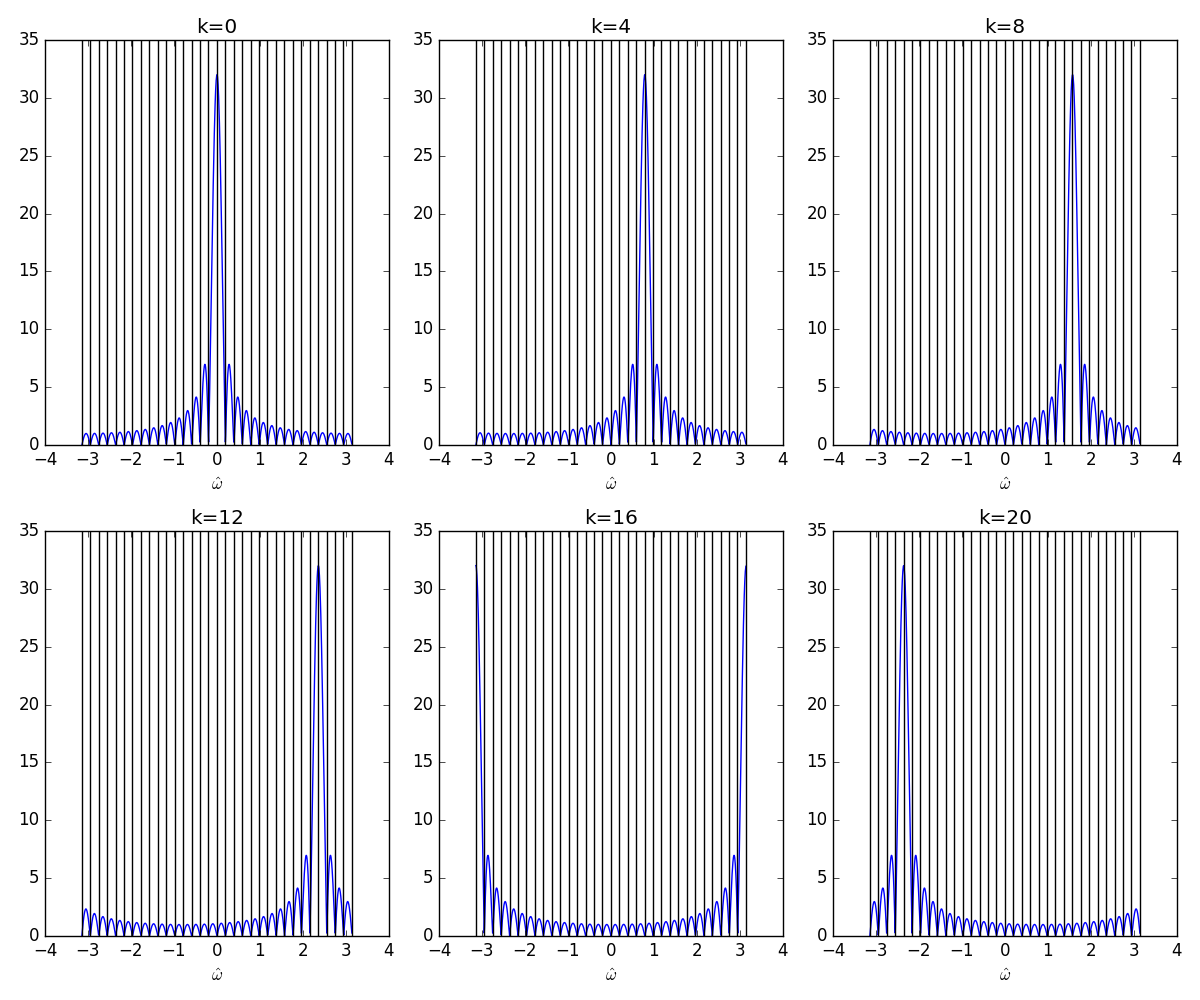
\includegraphics[width=\textwidth]{ch16/figures/fft_freqresp.png}
\end{center}
\caption{The magnitude response $|\mathcal{H}_k(\hat{\omega})|$ for several values of $k$. Each DFT output bin $\hat{x}[k]$ can be thought of as the output of a frequency selective filter with this magnitude response. For example, $k=0$ corresponds to a low-pass filter that passes mainly spectral components of the signal $x[n]$ that have a frequency close to zero.}
\label{fig:dft_freq_resp}
\end{figure}

From this plot, it is obvious that complex sinusoidal signals at
nearly all frequencies, except for frequencies $\hat{\omega}_{k}$, will
leak into the filter output with fairly significant amplitudes. This
is often unwanted.

\subsection{Windowed DFT}

In order to reduce the spectral sidelobes seen in
Figure \ref{fig:dft_freq_resp}, a tapered window function can be
used. The procedure is relatively simple. One applies a more selective
window function to the signal before evaluating the DFT. This is
equivalent to the tapered frequency selective filter shown in the
chapter on practical filters. The impulse response of each filter in
the filter bank will now be:
\begin{equation}
h_{R,k}[n] =\left\{ \begin{array}{cc}
w(N-1 + n)e^{i \frac{2\pi}{N}k n} & -(N-1) \le n \le 0\\
0 & \mathrm{otherwise}.
\end{array}
\right.
\end{equation}
Here $w(n)$ is a tapered window function of length $N$. 

The filter bank can now be implemented using a DFT as follows:
\begin{equation}
\boxed{
\hat{x}_w[k] = \sum_{n=0}^{N-1}x[n]w_N(n)e^{-i\frac{2\pi}{N}nk}.
}
\label{wdft}
\end{equation}
This results in a wider central peak at each frequency, but less
spectral leakage from signals outside frequency $\hat{\omega}_k$.

Figure \ref{fig:windowed_dft} shows the magnitude response
for several DFT frequency components below, when a Hann window
(Equation \ref{eq:hann_window_def}) of length $N=32$ is applied to the
signal:
\begin{figure}
\begin{center}
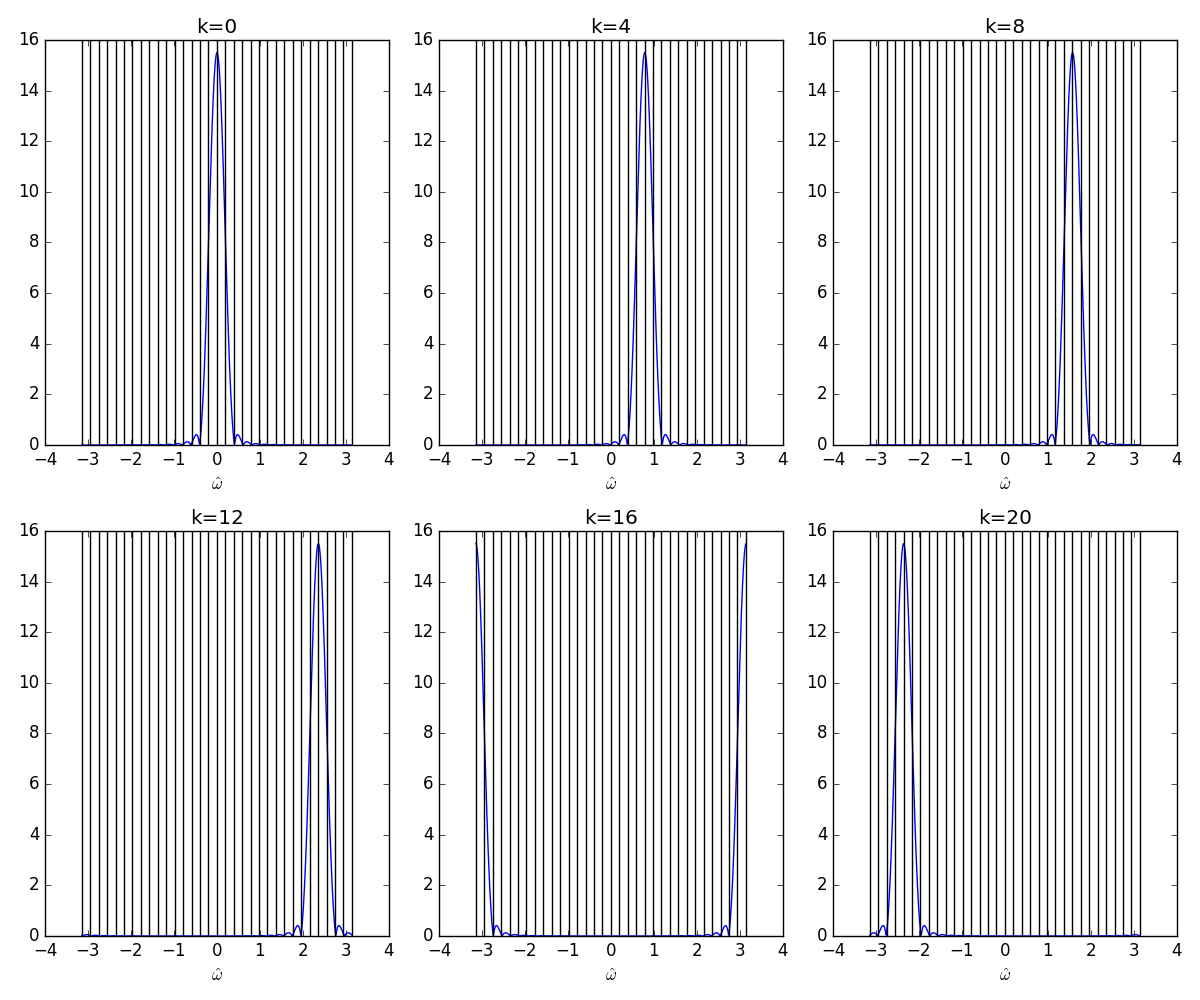
\includegraphics[width=\textwidth]{ch16/figures/fft_freqresp_w.png}
\end{center}
\caption{Windowed DFT filter bank $|\mathcal{H}_k(\hat{\omega})|$ magnitude responses for several values of $k$. 
Compared to rectangular window function, the magnitude response of the Hann windowed DFT filter bank has significantly lowered sidelobes. There is less out-of-band
signal leaking into the pass band of each frequency.}
\label{fig:windowed_dft}
\end{figure}

In nearly all spectral analysis applications, it is beneficial to
apply a window function to the signal that is being analyzed for
spectral content, to avoid spectral leakage.

\section{Example: Spectral analysis using windowed DFT}

The following example illustrates the advantages of using a window
function with low spectral sidelobes when using an FFT for spectral
analysis.

Let's generate a synthetic signal, which consists of a large and a small amplitude sinusoidal signal.
\begin{equation}
y[n] = A_1 \sin(\hat{\omega}_1 n) + A_2 \sin(\hat{\omega}_2 n),
\end{equation}
where $A_1 \gg A_2$ and $\hat{\omega}_1 \ne \hat{\omega}_2$. This signal is shown in
Figure \ref{fig:strong_weak_time}. When looking at the plot of the
signal $y[n]$ in time domain, it is very difficult, if not impossible,
to identify the weak signal. The strong signal overpowers it.

\begin{figure}
\begin{center}
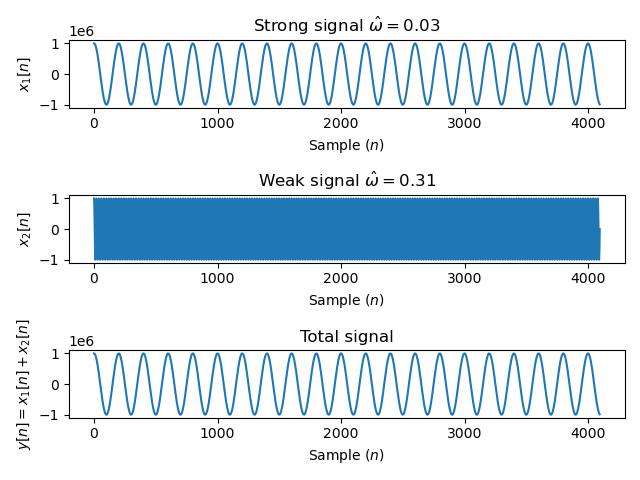
\includegraphics[width=\textwidth]{code/022_window_functions/windowed_signals.png}
\end{center}
\caption{Top: a large amplitude sinusoidal signal, Middle: a small amplitude sinusoidal signal. Bottom: Sum signal $y[n]$. When added together, the large amplitude signal dominates and the small amplitude signal cannot be visually detected.}
\label{fig:strong_weak_time}
\end{figure}

When analyzing the signal for spectral content using an unwindowed DFT, we get:
\begin{equation}
\hat{y}[k] = \sum_{n=0}^{N-1} y[n]e^{-i\frac{2\pi}{N}nk}.
\end{equation}
The strong sinusoidal signal $A_1 \sin(\hat{\omega}_1 n)$ will result
in a non-zero output for all spectral components $\hat{y}[k]$. This
``spectral'' leakage can easily overpower the weaker spectral
component. Power in decibel scale ($10 \log_{10}|\hat{y}[k]|^2$) is
shown with a blue line in
Figure \ref{fig:windowed_nonwindowed_spec}. It is easy to identify one
strong spectral peak corresponding to the large amplitude sinusoidal
signal with frequency $\hat{\omega}_1$.

In order to detect the sinusoidal signal with the small amplitude, we can use a windowed DFT:
\begin{equation}
\hat{y}_w[k] = \sum_{n=0}^{N-1} y[n]w(n)e^{-i\frac{2\pi}{N}nk}.
\end{equation}
Power in decibel scale is shown with an orange line in Figure \ref{fig:windowed_nonwindowed_spec}. In this
case, spectral leakage is reduced significantly, and it is possible to
identify the weak spectral component. 

\begin{figure}
\begin{center}
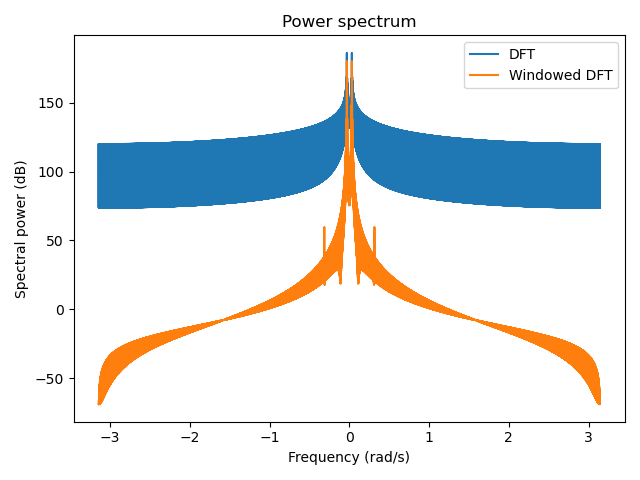
\includegraphics[width=\textwidth]{code/022_window_functions/windowed_spec.png}
\end{center}
\caption{Spectral power with (orange) and without (blue) a tapered window function. Without a tapering window, 
it is impossible to identify the sinusoidal signal with a very small amplitude, as spectral leakage from 
the large amplitude sinusoidal signal overpowers the weak signal.}
\label{fig:windowed_nonwindowed_spec}
\end{figure}

The Python program used to create the plots for this example is shown in Listing \ref{lst:windowed_dft}

\lstinputlisting[language=Python,caption={\texttt{022\_window\_functions/windowed\_dft.py}},label=lst:windowed_dft]{code/022_window_functions/windowed_dft.py}



\section{Example: Dynamic spectrum}

Signals are rarely unchanging in their spectral content. In many
applications, it is advantageous to analyze the time-frequency
evolution of signals. This can be done with the help of a windowed DFT
and selecting portions of the signal $x[n]$ of length $N$. This
results in a 2d signal, containing time and frequency:
\begin{equation}
\hat{x}[t,k] = \sum_{n=0}^{M-1} x[n+t\Delta n] w_N(n) e^{-i\frac{2\pi}{M}kn}.
\end{equation}
Here $\Delta n$ is the number of samples between spectral
estimates. This type of time-frequency spectrum is sometimes called
a \emph{\index{dynamic spectrum}{dynamic spectrum}} or
a \emph{\index{spectrogram}{spectrogram}}\sidenote{There is an implementation of a spectrogram in \texttt{scipy.signal.spectrogram}.}. 

Note that in this case, $N$ samples in time are used for each
spectrum, so the spectral estimate is not instantaneous, but an
average over $N$ samples. This is yet again a consequence of
time-frequency ambiguity.

Zero padding of the DFT to length $M$ can also be used to produce a
higher resolution DTFT estimate. In this case, $M$ denotes the length
of the DFT, and $w_N(n)$ indicates a window function of length $N$,
which will zero-pad samples of $x[n]$ at values of $n$ beyond sample
$N-1$.

An example of a dynamic spectrum is shown in
Figure \ref{fig:dynamic_spectrum_ex}. The signal that is analyzed in
time and frequency is a chirp signal:
\begin{equation}
x[n]=\sin(a n^2),
\end{equation}
which has a frequency that increases as a function of time.

The figure is produced with the Python program shown in
Listing \ref{lst:dynamic_spectrum} shown below, which implements
a dynamic spectrum using the FFT function in Python.

\begin{figure}
\begin{center}
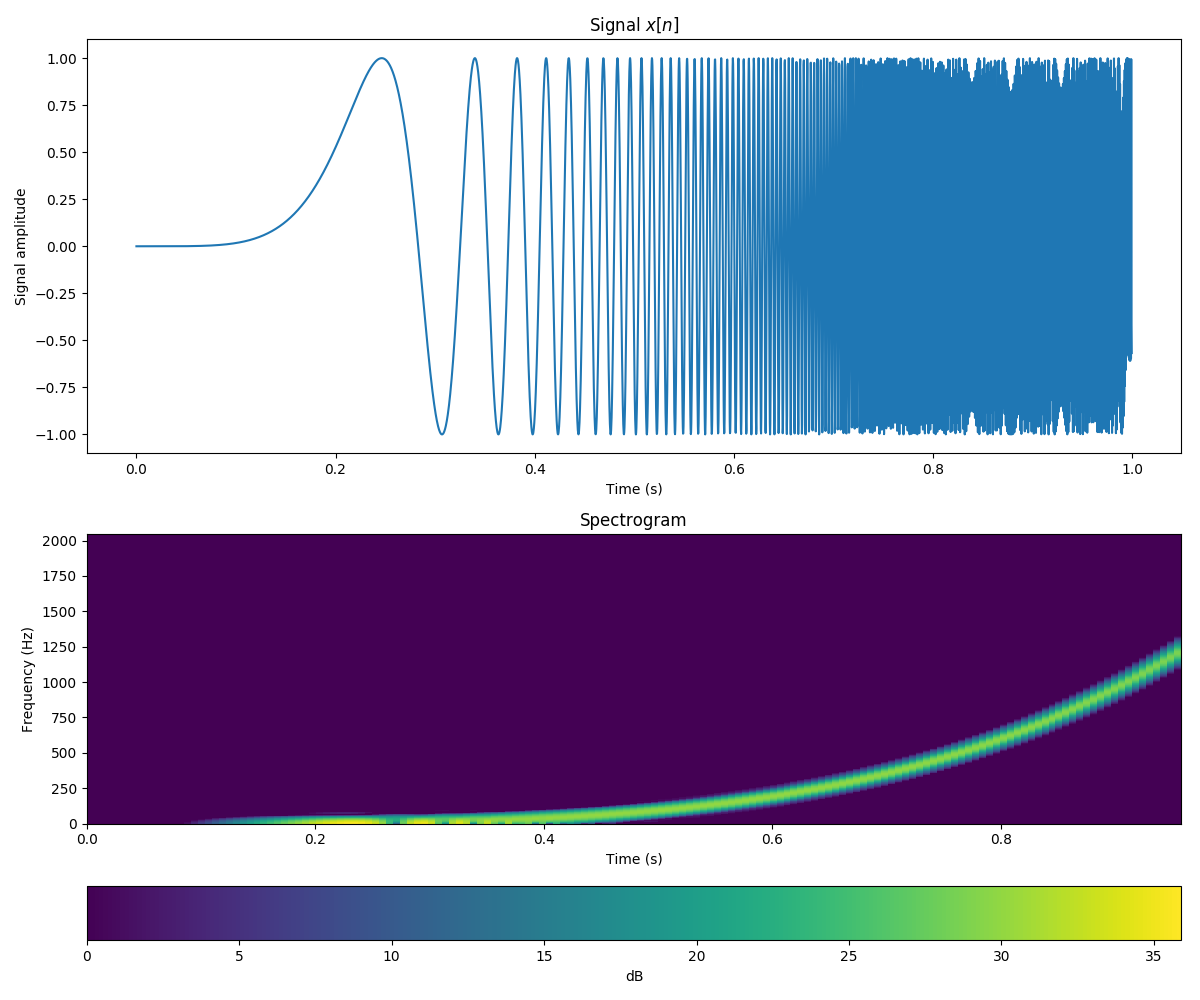
\includegraphics[width=\textwidth]{code/023_dynamic_spectrum/dynspec.png}
\end{center}
\caption{Time-frequency power spectrum $10 \log_{10}|X[t,k]|^2$ for a chirp signal, which increases in frequency.}
\label{fig:dynamic_spectrum_ex}
\end{figure}

\lstinputlisting[language=Python,caption={\texttt{023\_dynamic\_spectrum/dynamic\_spectrum.py}},label=lst:dynamic_spectrum]{code/023_dynamic_spectrum/dynamic_spectrum.py}



